We next consider a complex entire-muscle model involving motoneurons, sarcomeres and spindles.
The motoneurons and sarcomeres are used to model a \e{motorunit}, which is associated with a specific \e{fibre type} $\tau\in[0,1]$.
Here, $\tau=0$/$\tau=1$ corresponds to slow/fast twitch fibres, respectively.
We choose $\mups\in \N$ different motorunits in a ``motorunit-pool'', specified by $\tau_k\in[0,1], k=1\ldots\mups$.

\subsection{Motoneuron}
The motoneuron model \cite{Cisi2008, negro2011} consists of $6$ degrees of freedom and reads as
\begin{align}
	\vq'(t) &= \fmo(\vq(t),\tau) + \ve_2\kappa(t)\eta(t,\tau) + \ve_2\eta_b(t) & \vq(0) &= \vnull,
\end{align}
for any fibre type $\tau$.
Here, $\ve_2\in\R^6$ is the second unit-vector, $\eta(t,\tau),\eta_b(t)$ describe noises (fibre-type dependent and base noise)
and $\kappa(t)$ an external input signal (e.g. from the central cortex).
This is used to activate/stimulate the motoneuron by addition to the second component $\fmo_2$, which describes the voltage change on the cell's soma.
The external signal $\kappa(t)$ can be seen as a \e{mean current}, as it imitates the overloaded signal from many firing distant neurons.
We will use $\vq^k(t) \in \R^6$ to indicate the current state of the $k$-th motoneuron (of the $k$-th motorunit).

\fix{motoneuron model parameter interpolation (coolExp)}
\fix{maximum mean input current!}

\subsection{Sarcomere}
The sarcomere model describes the force development inside a muscle fibre and is taken from \cite{Shorten2007}.
It has $56$ degrees of freedom and is given by
\begin{align}
	\vr'(t) &= \fsa(\vr(t),\tau) & \vr(0) &= \vr_0(\tau),
\end{align}
for any fibre type $\tau$.
There is a set of $105$ (fibre-type dependent) constants for the model, which we denote by $\csa(\tau)\in\R^{105}$.
We denote by $\vr^k(t)\in\R^{56}$ the state of the $k$-th sarcomere model (of the $k$-th motorunit).

\subsection{Spindle}
The spindle is the muscle component responsible for motoneuron feedback, where the model used is from \cite{Mileusnic2006}.
It has $9$ degrees of freedom and is given by
\begin{align}
	\vs'(t) &= \fsp(\vs(t),\dla(t),\nu(t)) & \vs(0) &= \vnull,\label{def:spindlesys}
\end{align}
where $\dla$ describes the change in fibre length and $\nu$ the frequency of an associated motoneuron.
We denote by $\vs^k(t)\in\R^9$ the state of the $k$-th spindle model. In real muscles, the number of spindles is independent from the
number of motorunits, but we use $\mups$ here for simplicity.

\subsection{Model connections}
As the models have not been primarily designed to be used in a compound, we needed to develop appropriate means for their connection.
In this Section we will detail how the different models have been connected.

%
\begin{figure}[!htp]
    \begin{center}%
    \begin{tikzpicture}[auto,%
            block_assign/.style ={rectangle, draw=black, very thick, fill=white,%
            text width=10em, text centered, minimum height=3em, inner sep=6pt},%
            block_big/.style ={rectangle, draw=black, very thick, fill=white,%
            text width=14em, text centered, minimum height=3em, inner sep=6pt},%
            block_dashed/.style ={rectangle, draw=black, very thick, fill=white,%
            text width=10em, text centered, minimum height=3em, inner sep=6pt},%
        ]%
        \tikzstyle{stateEdgePortion} = [black, very thick, -latex', shorten >=1pt];
        \tikzstyle{stateEdge} = [stateEdgePortion];
        \tikzstyle{edgeLabel} = [pos=0.5, text centered];
        \tikzstyle{edgeLabelLow} = [pos=0.25, text centered];
        \tikzstyle{edgeLabelHigh} = [pos=0.25, text centered];
        \tikzstyle{line} = [draw, black, very thick, -latex', shorten >=1pt]];
        \tikzstyle{sline} = [draw, black, very thick];
        \tikzstyle{dline} = [draw, black, dashed, very thick, -latex', shorten >=1pt]];
        \tikzstyle{doublearrow} = [draw, black, very thick, <->, -latex', shorten >=1pt, shorten <=5pt, >=stealth]];
%        \tikzstyle{doubledline} = [draw, black, dashed, very thick, <->, -latex', shorten >=1pt, shorten <=5pt, >=stealth]];
        \node [block_big] (neuro)  {{\bf motoneurons} $\vq^k(t)$\\firing times, spindle feedback};%
        \node [block_big, below of=neuro, node distance=30mm] (cell)  {{\bf half-sarcomeres $\vr^k(t)$}\\ action potential, active stress};%
        \node [block_big, above of=neuro, node distance=30mm] (ext)  {{\bf External signal}\\ Control, central cortex};%
        \node [block_dashed, left of=cell, node distance=80mm] (spindle)  {{\bf spindles $\vs^k(t)$} \\ electrical feedback};%
        \node [block_big, below of=cell, node distance=30mm] (mechanics)  {{\bf 3D continuum mechanics} \\ geometry, deformation};%
        \path [line] (neuro) -- (cell) node[edgeLabel]{$q^k_2(t)$};
        \draw (cell.south) edge[stateEdge] node[edgeLabel]{$\alpha(X,t)$} (mechanics.north);
        \path [line] (mechanics) -| (spindle) node[edgeLabelHigh]{$\dla(X_k),\la''(X_k)$};
    	\path [line] ($(neuro.west) + (0,0.3)$) -| ($(spindle.north) + (-0.5,0)$);
    	\path [line] ($(spindle.north) + (0.5,0)$) |- ($(neuro.west) + (0,-0.3)$);
    	\path [line] (ext) -- (neuro.north) node[edgeLabel] {$\kappa(t),\eta(t),\eta_b(t)$}; 
      	\node at (-5.7,-0.7) {$\kappa^s(t)$};
    	\node at (-5.8,0.8) {$\kappa(q^k_2(t))$};
    \end{tikzpicture}%
    \end{center}%
    \caption{Test}
\end{figure}

\subsubsection{Motoneuron to Sarcomere}
The motoneuron soma signals $q^k_2(t)$ are used to provide activation spikes for the $k$-th sarcomere.
As the sarcomere model merely reacts to high spikes, the motoneuron output is scaled by a nonlinear function $\gamma$ to emphasize high peaks.
Essentially, the small signals are multiplied by a small factor $\beta_m = 0.3$, and the high signals are intensified by $\beta_M = 7$.
The transition from low to high factor is realized by a smooth Gaussian,
where we choose a threshold signal of $q_M = 40$ to pinpoint the signal from which on the $\beta_M$ factor is applied:
\begin{align}
	\gamma(q) &:= \begin{cases}
		\beta_m + e^{-(q-q_M)^2/150}(\beta_M-\beta_m), & 0 < q < q_M\\
		\beta_M & q \geq q_M,
	\end{cases}
\end{align}
Figure \ref{MSLink} illustrates the 
\begin{figure}[!ht]
	\centering
	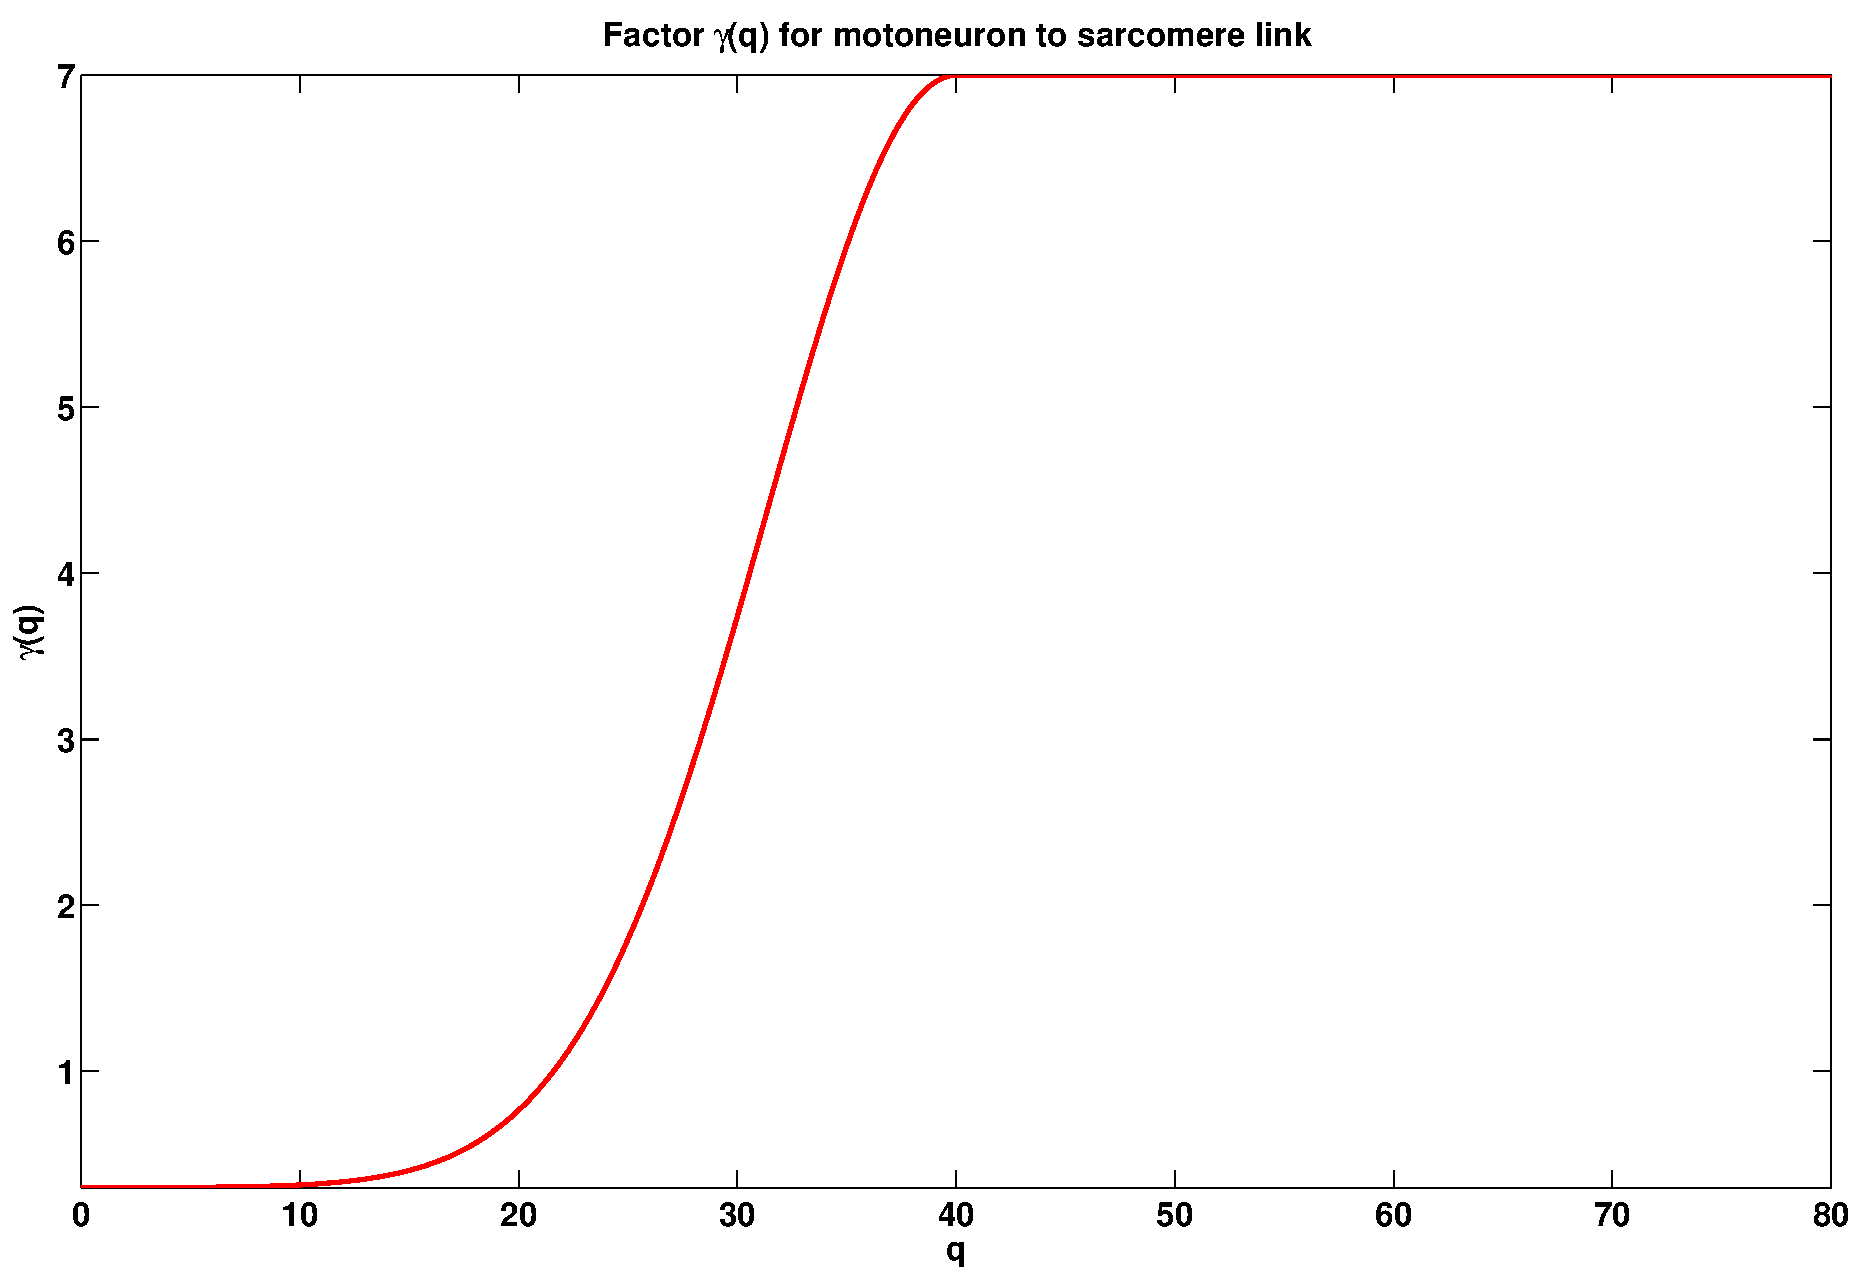
\includegraphics[width=\single]{moto_sarco_link_factor.pdf}
	\caption{Amplification factor for motoneuron signals}
	\label{fig:MSLink}
\end{figure}
Taking into account division by sarcomere model constants, the sarcomere models now read as
\begin{align}
	{\vr'}^k(t) &= \fsa(\vr^k(t),\tau_k) + \ve_1 \frac{\gamma(q_2^k(t))}{\csa_1(\tau_k)}q_2^k(t),
\end{align}
where $\ve_1 \in \R^{56}$ denotes the first unit vector, i.e. the signal is added to the first component of the sarcomere models.

\subsubsection{Sarcomere to Mechanics}
The sarcomere model component $\vr_{53}^k(t)$ is an indicator for the currently developed force in the muscle fibre.
\fix{hier das modell aus der diss erwähnen mit fasern und diffusion + erläuterung}
Within the mechanics FE-framework, this can be transformed to active stress $\alpha(X,t)$ in $\vSf$ by weighting of all $\mups$ force signals at spatial locations.
Hence, we make the ansatz
\begin{align}
	\alpha(X,t) = \sum\limits_{k=1}^\mups \frac{w_k(X)}{r^k_M} r^k_{53}(t).
\end{align}
Here, we introduce weight functions $w_k(X)$ for the fibre forces satisfying $\sum w_k(X) = 1 \fo X$.
Further, the constants $r^k_M\in\R$ are the maximum forces for each motorunit (i.e. $\tau_k$), determined by a long-time simulation of each sarcomere model using an
artificial $60Hz$ stimulation.
This ensures that $\alpha(X,t) \in [0,1] \fo X,t$. 

\subsubsection{Mechanics to Spindle}
According to \ref{def:spindlesys}, the spindle models use two external inputs:
The current change rate $\dla$ of fibre stretch and the motoneuron frequency $\kappa(t)$, where the latter will be discussed in Section
\ref{subsec:moto_spindle}.
As the fibre stretch is a local property of the continuum, we fix $\mups$ spindle locations $X_k\in\Omega$ and simply observe $\dla(X_k,t)$ to obtain the second
argument of the $k$-th spindle dynamics $\fsp$.
We recall the definition \ref{def:fibrestretch} and observe 
\begin{align*}
	\dla(X,t) &= \d{}{t}\no{\vF(X,t)\va_0(X)} = \frac{(\vF(X,t)\va_0(X))^T}{\no{\vF(X,t)\va_0(X)}}\d{}{t}\vF(X,t)\va_0(X)\\
	  &= \frac{1}{\la(X,t)}\va_0(X)^T\vF(X,t)^T\vF'(X,t)\va_0(X).
\end{align*}
Hence, if the $X_k$ are chosen among the set of all elements' Gauss integration points, quantities to compute $\dla$ are readily available during mechanics evaluation.

\subsubsection{Spindle to Motoneuron}
According to \cite{Mileusnic2006}, the spindle model has two algebraic scalar quantities called \e{primary} and \e{secondary afferents},
denoted by $\theta_p(\vs^k(t))$ and $\theta_s(\vs^k(t))$, respectively.
These afferents describe the firing frequency in [pps] of the spindle dendrites leading back into the motoneuron pool.
In a muscle, all spindles are connected to the entirety of the motoneuron pool \fix{ref?}, which will be modeled via averaging of all $\mups$ spindle's afferent outputs.
This gives a \e{mean spindle activation} of
\begin{align}
	\kappa^s(t) &:= \frac{1}{\mups}\sumjmups w_p\theta_p(\vs^j(t)) + w_s\theta_s(\vs^j(t))
\end{align}
which is added to the change rate of each motoneuron's soma alike the external mean current:
\begin{align}
	\vq'(t) &= \fmo(\vq(t),\tau) + \ve_2(\kappa(t) + \kappa^s(t))\eta(t,\tau) + \ve_2\eta_b(t).
\end{align}    
% [6{:}8] , where the \ML-like notation indicates which components of the spindle states $\vs$ are used as arguments.

\subsubsection{Motoneuron to Spindle}\label{subsec:moto_spindle}
In order to provide the Spindle model with the current motoneuron frequency, the discrete signal $s_n := q^k_2(t_n)$ at times $t_n, t_1 < t_2 < t_3 \ldots$ needs to be converted to
a frequency $\nu_n$.
Essentially, the last $W \in\N$ peaks are tracked and the frequency is determined by the time elapsed between the last $W$ peaks.    
This is done by a simple automata described in Figure \ref{fig:FD}, where we have two thresholds $p^+,p^-$ denoting the start and end of a peak, respectively.
\begin{figure}[!ht]
    \centering
	\begin{tikzpicture}[shorten >= 2pt, node distance=2cm, auto]
		\node (S) at (-.5,0) {start};
		\node[state] (poff) at (1,0) {$P_-$};
		\node[state] (pon) at (4,0) {$P_+$};
		\path[->] (S) edge node {} (poff)
				  (poff) edge[out=40,in=140] node[above] {$s_n > p^+$} (pon)
				  (pon) edge[out=40,in=320,looseness=4] node[right] {$s_n > p^-$} (pon)
				  (pon) edge[out=220,in=320] node[below] {$s_n < p^-$} (poff);
	\end{tikzpicture}
    \caption{Frequency-detection automata}\label{fig:FD}
\end{figure}
Whenever the transition from $P_-$ to $P_+$ is done, the ``peak counter'' $k$ (starting from $k=0$) is increased by one and the current time $t_n$ is stored via $t^p_k = t_n$.
Then the frequency sequence is then given by
\begin{align}
	\nu_n &:= \begin{cases}
		\frac{W}{t_n - t^p_{k-W}} & k \geq W,\\
		0 & k < W.
	\end{cases}
\end{align}
As the detector essentially computes a local average over $W$ peaks, a larger ``window size'' $W$ improves accuracy with respect to a noisy signal,
while a smaller $W$ renders the detector more sensitive to quick frequency changes.
In our applications $W=3$ or $W=4$ turned out to be appropriate choices.

\subsubsection{Model parameters}
\begin{table}[!ht]
	\begin{tabular}{l|l|l}
		Name & Value & Context\\\hline
		$\beta_m$ & 0.3 & Moto-Sarco link min factor\\
		$\beta_M$ & 7 & Moto-Sarco link max factor\\
		$q_M$ & 40 & Moto-Sarco link max factor signal\\
		$w_p$ & 0.002 & Primary afferent weight\\
		$w_s$ & 0.002 & Secondary afferent weight\\
		$p^+$ & 40 & Frequency detector ``peak on'' threshold\\
		$p^-$ & 15 & Frequency detector ``peak off'' threshold\\
		$W$ & 3-4 & Frequency detector peak window size
	\end{tabular}
	\caption{Model-related parameters}\label{tab:params}
\end{table}
\begin{table}[!ht]
	\begin{tabular}{l|ll}
		Name & Context\\\hline
		$r^k_M$ & Maximum force response of single sarcomere at constant, full activation ($60Hz$) 
	\end{tabular}
	\caption{Experimentally determined quantities}\label{tab:params}
\end{table}
\begin{table}[!ht]
	\begin{tabular}{l|ll}
		Name &  Context\\\hline
		$w_k$ & Weights for fibre forces at each Gauss point  
	\end{tabular}
	\caption{Model design variables}\label{tab:params}
\end{table}
